\begin{knitrout}
\definecolor{shadecolor}{rgb}{1, 1, 1}\color{fgcolor}\begin{kframe}
\begin{alltt}
\hlkwd{library}\hlstd{(KernSmooth)}

\hlstd{fhat_normal} \hlkwb{<-} \hlkwd{bkde}\hlstd{(x,} \hlkwc{kernel} \hlstd{=} \hlstr{"normal"}\hlstd{,} \hlkwc{bandwidth} \hlstd{=} \hlnum{0.05}\hlstd{)}
\hlkwd{plot}\hlstd{(fhat_normal,} \hlkwc{type} \hlstd{=} \hlstr{"l"}\hlstd{)}
\end{alltt}
\end{kframe}
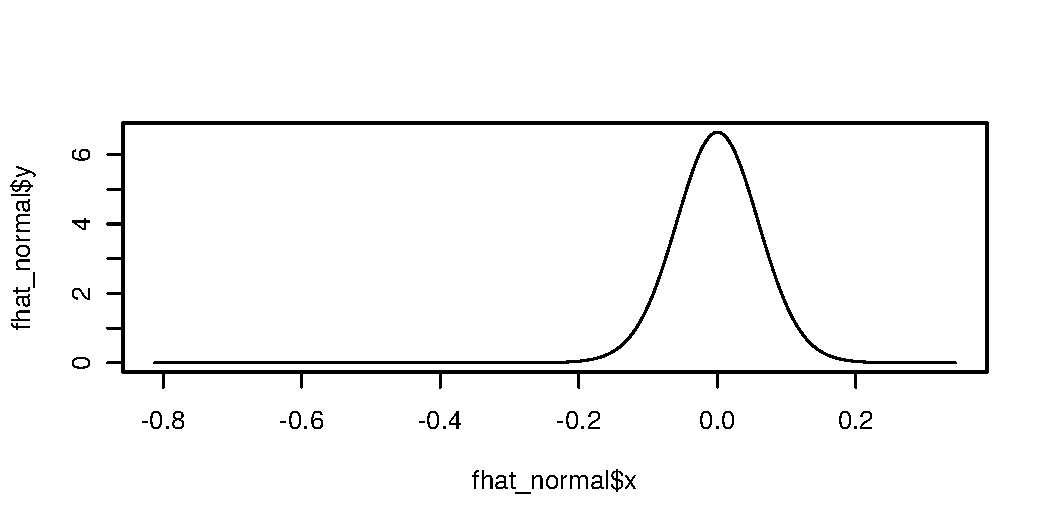
\includegraphics[width=\maxwidth]{figure/unnamed-chunk-17-1} 
\begin{kframe}\begin{alltt}
\hlstd{fhat_unif} \hlkwb{<-} \hlkwd{bkde}\hlstd{(x,} \hlkwc{kernel} \hlstd{=} \hlstr{"box"}\hlstd{,} \hlkwc{bandwidth} \hlstd{=} \hlnum{0.05}\hlstd{)}
\hlkwd{plot}\hlstd{(fhat_unif,} \hlkwc{type} \hlstd{=} \hlstr{"l"}\hlstd{)}
\end{alltt}
\end{kframe}
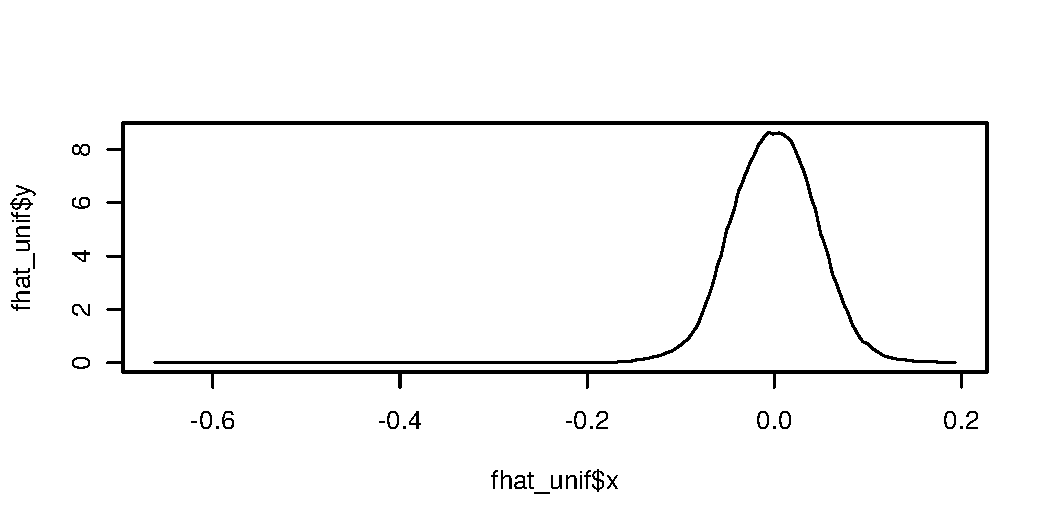
\includegraphics[width=\maxwidth]{figure/unnamed-chunk-17-2} 
\begin{kframe}\begin{alltt}
\hlstd{fhat_epanech} \hlkwb{<-} \hlkwd{bkde}\hlstd{(x,} \hlkwc{kernel} \hlstd{=} \hlstr{"epanech"}\hlstd{,} \hlkwc{bandwidth} \hlstd{=} \hlnum{0.05}\hlstd{)}
\hlkwd{plot}\hlstd{(fhat_epanech,} \hlkwc{type} \hlstd{=} \hlstr{"l"}\hlstd{)}
\end{alltt}
\end{kframe}
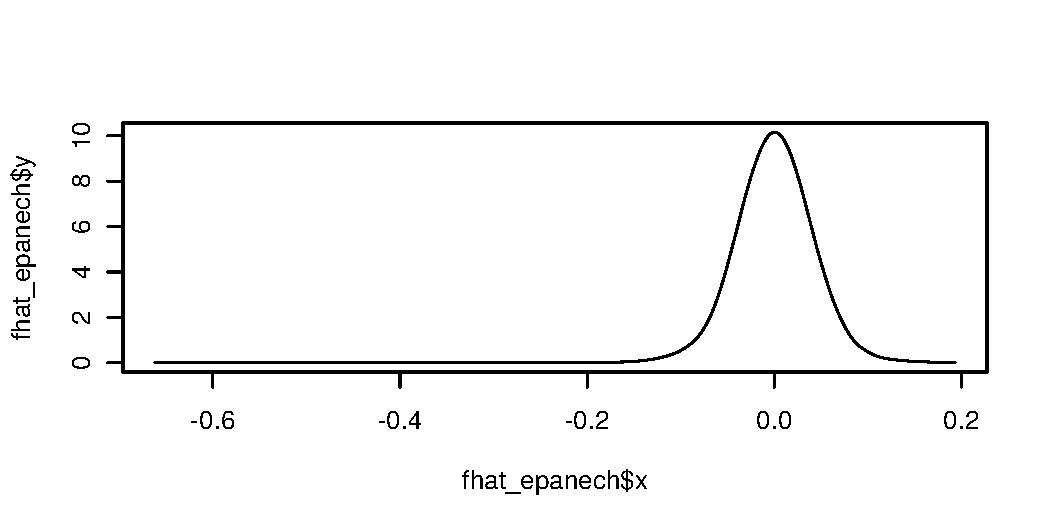
\includegraphics[width=\maxwidth]{figure/unnamed-chunk-17-3} 
\begin{kframe}\begin{alltt}
\hlstd{fhat_biweight} \hlkwb{<-} \hlkwd{bkde}\hlstd{(x,} \hlkwc{kernel} \hlstd{=} \hlstr{"biweight"}\hlstd{,} \hlkwc{bandwidth} \hlstd{=} \hlnum{0.05}\hlstd{)}
\hlkwd{plot}\hlstd{(fhat_biweight,} \hlkwc{type} \hlstd{=} \hlstr{"l"}\hlstd{)}
\end{alltt}
\end{kframe}
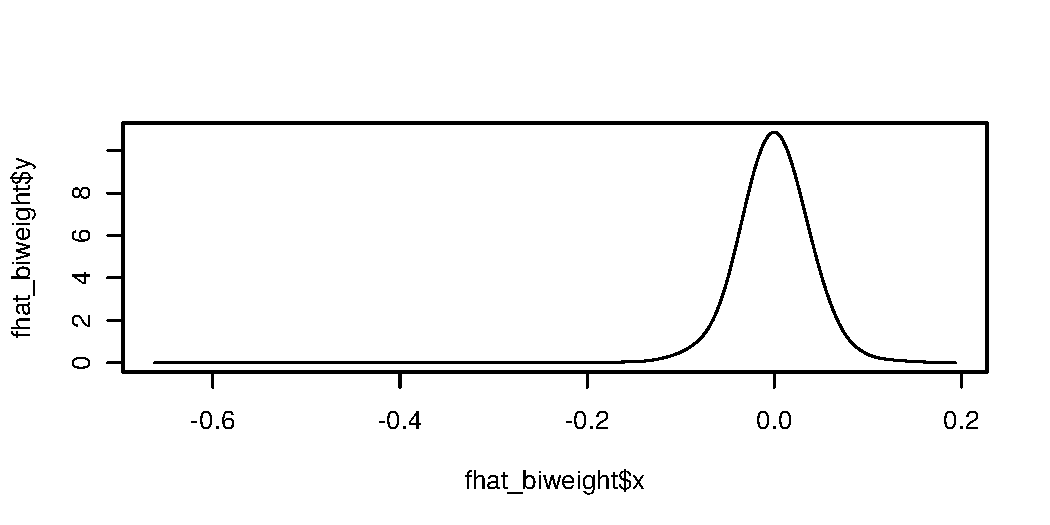
\includegraphics[width=\maxwidth]{figure/unnamed-chunk-17-4} 
\begin{kframe}\begin{alltt}
\hlstd{fhat_triweight} \hlkwb{<-} \hlkwd{bkde}\hlstd{(x,} \hlkwc{kernel} \hlstd{=} \hlstr{"triweight"}\hlstd{,} \hlkwc{bandwidth} \hlstd{=} \hlnum{0.05}\hlstd{)}
\hlkwd{plot}\hlstd{(fhat_triweight,} \hlkwc{type} \hlstd{=} \hlstr{"l"}\hlstd{)}
\end{alltt}
\end{kframe}
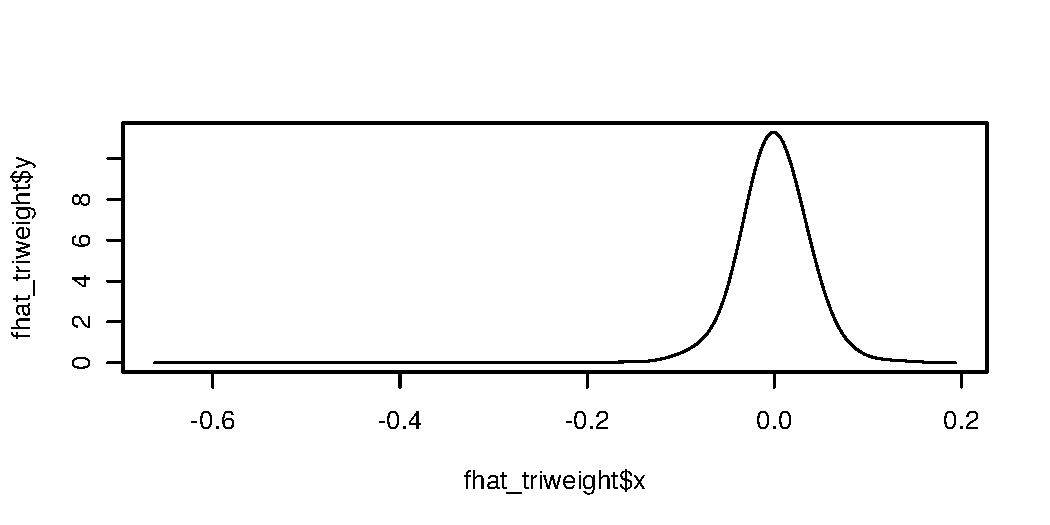
\includegraphics[width=\maxwidth]{figure/unnamed-chunk-17-5} 

\end{knitrout}
